\documentclass[tikz,border=10pt]{standalone}
\usetikzlibrary{angles}
\begin{document}
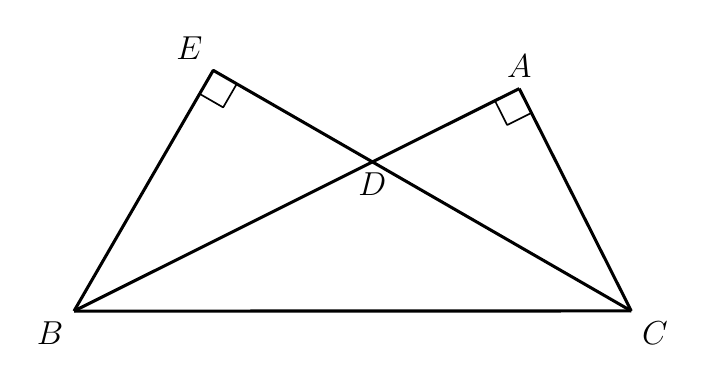
\begin{tikzpicture}[line join=round, line width=1.1pt, font=\fontsize{11.5}{13.8}\selectfont]
\coordinate (A) at (2.116,1.156);
\coordinate (B) at (-3.538,-1.669);
\coordinate (C) at (3.539,-1.668);
\coordinate (D) at (0.252,0.225);
\coordinate (E) at (-1.770,1.388);




\draw (B) -- (C);
\draw (B) -- (D) -- (A);
\draw (C) -- (A);
\draw (B) -- (E) -- (D) -- (C);


\draw pic[draw, line width=0.6pt, angle radius=0.345cm] {right angle=B--A--C};
\draw pic[draw, line width=0.6pt, angle radius=0.345cm] {right angle=B--E--C};


\node[below left] at (B) {$B$};
\node[below right] at (C) {$C$};
\node[above] at (A) {$A$};
\node[above left] at (E) {$E$};
\node[below] at (D) {$D$};
\end{tikzpicture}
\end{document}